\section{Efficiency} 
  
\subsection{Classification of Decision Problems}

  We have talked about \textit{optimization problems} that choose the best solution from a class of solutions. Now we will talk about \textit{decision problems}, which seek to prove or disprove the existence of a solution satisfying a certain property. 

  \begin{lemma}[Conversion between Optimization and Decision Problems]
    It turns out we can convert one into the other easily by rephrasing the problem. The following conversion will be used frequently.  
    \begin{enumerate}
      \item Given a problem $P$, we want to find a solution that minimizes some variable $K$. 
      \item Given a problem $P$ and some constant $K^\prime$, does there exist a solution that is less than $K^\prime$? 
    \end{enumerate}
    Voila.  
  \end{lemma}

  Now that this is established, we can freely consider the classes P and NP of all decision problems and classify them. There are equivalent definitions for optimization problems, but it is more popular to pose these classes as decision problems. 

  \begin{definition}[P]
    $P$ (Polynomial Time) is the set of all decision problems that can be solved by polynomial-time algorithms. 
  \end{definition} 

  \begin{definition}[NP]
    $NP$ (Nondeterministic Polynomial Time) is the set of all decision problems for which if it returns $1$ (i.e. a solution exists), this can be \textit{verified} in polynomial time.\footnote{The fact that a \textit{proposed} solution can be verified is important! Proving or disproving a proposed solution is much easier than proving the nonexistence of a solution.}
  \end{definition}

  The other way around $NP \subset P$ is an unsolved millenium conjecture. It attempts to answer what the runtime difference or difficulty is between solving and verifying a problem? The conjecture states that solving is exponentially harder that verifying. 

  \begin{theorem}
    $P \subset NP$
  \end{theorem}
  \begin{proof}
    Given a problem $\pi$ with a proposed solution $p$, we can run $p$ in polynomial time to verify it. 
  \end{proof}

  Colloquially, the set of problems which are at least as hard as NP is called \textit{NP-hard}, which can be defined for both optimization and decision problems. These are the absolute hardest problems. The formal definition of NP-Hard problems is shown below. 

  \begin{definition}[NP-Hard]
    A (decision or optimization) problem $\pi$ is NP-hard iff the existence of a polynomial time algorithm for $\pi$ implies $P = NP$. 
  \end{definition}

  \begin{definition}[NP-Complete]
    The intersection of NP-hard and NP is \textbf{NP-complete}, which can be thought of as the hardest problems existing in NP. The worst case runtime complexity of an NP-complete problem is exponential. 
  \end{definition}

  \begin{figure}[H]
    \centering 
    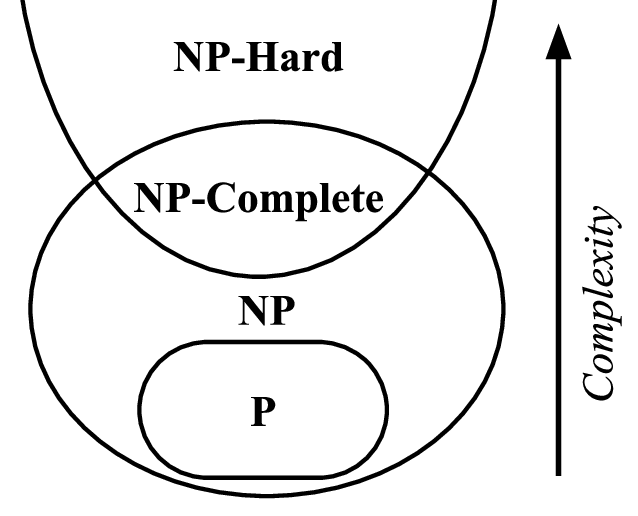
\includegraphics[scale=0.3]{img/class.png}
    \caption{Diagram of the 4 classes. The complexity rises as we go up. } 
    \label{fig:class}
  \end{figure}
  
\subsection{Proving NP-Hardness}

  To show that a problem is in P, all we have to do is find a polynomial time algorithm, which is what we've been doing this entire course. To show whether a problem is NP, we should show that it is verifiable in polynomial time, which we have also done so far. Proving NP-hardness (which then allows us to prove NP-completeness) is a bit more tricky. The pattern is always three things. 
  \begin{enumerate}
    \item \textit{Reduction}. Describe a polynomial time algorithm $f$ to transform an \textit{arbitrary instance} $x$ of a problem $\beta$ into a \textit{special instance} $y = f(x)$ of a problem $\pi$. 
    \item \textit{Equivalence}. Prove that if arbitrary $x$ is a true instance of $\pi$, then $y$ is a true instance of $\pi$. 
    \item \textit{Equivalence}. Prove that if arbitrary $y$ is a true instance of $\pi$, then $x$ is a true instance of $\pi$.\footnote{This is the hard part.} 
  \end{enumerate}

  \begin{definition}[Reduction]
    In other words, to prove a problem $\pi$ is NP-hard, reduce\footnote{The fact that we say reduce here is misleading, since we are showing that the reduction is at least as hard as the original.} a known NP-hard problem $\beta$ to $\pi$ in polynomial time (not the other way around!). If this reduction is possible, then we claim that $\pi$ must be at least as hard as $\beta$: $\beta \leq_p \pi$. 
    \begin{enumerate}
      \item Assume that we can solve $\pi$ in polytime. 
      \item Then we can solve $\beta$ in polytime by first converting any instance of $\beta$ to $\pi$ in polytime, and then polytime solving $\pi$.\footnote{In other words, there exists an injective (but not necessarily surjective) mapping from the set of solutions of $\pi$ to the set of solutions of $\beta$. }
      \item Therefore, $\pi \in P \implies \beta \in P$. 
    \end{enumerate}
    But since we already know $\beta$ is NP-hard, this creates a contradiction. Therefore, $\pi \not\in P$. 
  \end{definition}

  The reduction serves to compare the two problems, and the equivalence then serves to compare the set of solutions to these two problems.   

  \begin{definition}[Equivalence of Solutions]
    The next step is to show two things: 
    \begin{enumerate}
      \item A solution to $\pi$ implies a solution to $\beta$, and 
      \item A solution to $\beta$ implies a solution to $\pi$. 
    \end{enumerate}
  \end{definition} 

  As a general overview of popular problems and their relation to each other, we'll mention this now. 

  \begin{theorem}[Reduction Tree of NP-Hard Problems]
    For convenience. 
    \begin{enumerate}
      \item 3SAT is NP-hard by Cook-Levin 
      \item CircuitSAT is NP-hard by reducing from 3SAT 
      \item Max Independent Set is NP-hard by reducing from 3SAT 
      \item Min Vertex Cover is NP-hard by reducing from MIS 
      \item Max Clique is NP-hard by reducing from MIS \label{max-clique-np-hard}
      \item Hamiltonian Path is NP-hard 
      \item Hamiltonian Cycle is NP-hard by reducing from MVC, 3SAT, or Hamiltonian Path 
      \item Graph Coloring is NP-hard by reducing from 3SAT 
      \item Subset Sum is NP-hard by reducing from MVC 
      \item Planar CircuitSAT is NP-hard by reducing from CircuitSAT 
      \item Paritioning\footnote{Given a set $S$ of $n$ integers, are there disjoint subsets $A, B$ s.t. their sums are equal?} is NP-hard by reducing from Subset Sum. 
      \item Set Cover\footnote{Given a collection of sets $S$, find the smallest sub-collection of sets that contains all the elements in $\cup S$.} is NP-hard. 
      \item Longest Path is NP-hard. 
      \item MaxCut\footnote{Find the max cut of a graph.} is NP-hard. 
    \end{enumerate}
  \end{theorem}

\subsection{Logic and Satisfiability}

  \begin{definition}[CircuitSAT]
    Consider a black box circuit $f$, with input $\mathbf{x} \in \{0, 1\}^n$. We want to answer the question of whether there exists some $\mathbf{x}$ s.t. $f(\mathbf{x}) = 1$, i.e. whether the circuit is \textbf{satisfiable} (i.e. outputs a 1 bit). 

    \begin{figure}[H]
      \centering 
      \begin{tikzpicture}[scale=1.0]
        % Input labels
        \node (x1) at (0,3) {$x_1$};
        \node (x2) at (0,2) {$x_2$};
        \node (x3) at (0,1) {$x_3$};

        % NOT gate for x1
        \node[american not port, scale=0.7] (not1) at (2,3) {};

        % AND gate
        \node[american and port, scale=0.7] (and1) at (4,2.5) {};

        % OR gate
        \node[american or port, scale=0.7] (or1) at (6,1.5) {};

        % Final output
        \node (out) at (8,1.5) {$f(x_1,x_2,x_3)$};

        % Connections
        % x1 to NOT gate
        \draw (x1) -- (not1.in);
        
        % NOT output to AND input 1
        \draw (not1.out) -- ++(0.5,0) |- (and1.in 1);
        
        % x2 to AND input 2
        \draw (x2) -- ++(3,0) |- (and1.in 2);
        
        % AND output to OR input 1
        \draw (and1.out) -- ++(0.5,0) |- (or1.in 1);
        
        % x3 to OR input 2
        \draw (x3) -- ++(5,0) |- (or1.in 2);
        
        % OR output to final output
        \draw (or1.out) -- (out);

        % Gate reference symbols at bottom
        % AND gate reference
        \node[american and port, scale=0.7] (and-ref) at (2,-1) {};
        \node (and-x) at (1,-0.8) {$x$};
        \node (and-y) at (1,-1.2) {$y$};
        \node (and-out) at (3,-1) {$x \wedge y$};

        % OR gate reference
        \node[american or port, scale=0.7] (or-ref) at (5,-1) {};
        \node (or-x) at (4,-0.8) {$x$};
        \node (or-y) at (4,-1.2) {$y$};
        \node (or-out) at (6,-1) {$x \vee y$};

        % NOT gate reference
        \node[american not port, scale=0.7] (not-ref) at (8,-1) {};
        \node (not-x) at (7,-1) {$x$};
        \node (not-out) at (9,-1) {$\neg x$};

        % Connections for reference gates
        \draw (and-x) -- (and-ref.in 1);
        \draw (and-y) -- (and-ref.in 2);
        \draw (and-ref.out) -- (and-out);

        \draw (or-x) -- (or-ref.in 1);
        \draw (or-y) -- (or-ref.in 2);
        \draw (or-ref.out) -- (or-out);

        \draw (not-x) -- (not-ref.in);
        \draw (not-ref.out) -- (not-out);
      \end{tikzpicture}
      \caption{Some random circuit where $n = 5$.} 
      \label{fig:random_circuit}
    \end{figure}

    The obvious way is to brute force is an check all $2^n$ combinations, and this is the only way since this is black-box. However, even if we knew the circuit itself, the amount of computations that we need to solve this is conjectured to be still $O(2^n)$, though we may be able to cleverly shave off some calculations here and there.\footnote{It is not proven that there exists no exponential algorithm.}
  \end{definition}

  \begin{definition}[3SAT]
    Given a boolean formula $\phi$ of $N$ variables where each \textbf{clause} contains exactly 3 literals, determine if there exists a satisfying assignment to the variables that makes $\phi$ true. Formally:
    \begin{align*}
      \phi &= C_1 \land C_2 \land \cdots \land C_m \\
      C_i &= (l_{i1} \lor l_{i2} \lor l_{i3}) \\
      l_{ij} &\in \{x_k, \neg x_k\} \text{ for some } k \in \{1,\ldots,n\}
    \end{align*}
    where $x_k$ are boolean variables and $\neg x_k$ their negations. For example:
    \begin{align*}
      \phi = (x_1 \lor \neg x_2 \lor x_3) \land (\neg x_1 \lor x_2 \lor x_4) \land (x_2 \lor \neg x_3 \lor \neg x_4)
    \end{align*}
    Like CircuitSAT, this problem is also believed to require $O(2^n)$ time, and in fact these problems are polynomially reducible to each other (CircuitSAT $\leq_p$ 3SAT and 3SAT $\leq_p$ CircuitSAT). The key difference is that 3SAT has a very specific structure that makes it easier to analyze and reduce other problems to, making it a canonical NP-complete problem.\footnote{The restriction to exactly 3 literals per clause is not arbitrary - 2SAT is solvable in polynomial time, while 3SAT is NP-complete.}
  \end{definition}

  In fact, there is a polynomial time algorithm to translate between 3SAT and CircuitSAT, so the two are theoretically equivalent. 

  \begin{theorem}[P, NP Classification of SAT]
    For CircuitSAT, 
    \begin{equation}
      \texttt{CircuitSAT} \not\in P, \texttt{CircuitSAT} \in NP
    \end{equation}
    That is, it cannot be solved in polynomial time, but given a solution circuit and a satisfying assignment, the assignment can be verified in polynomial time. 
    For 3SAT, 
    \begin{equation}
      \texttt{3SAT} \not\in P, \texttt{3SAT} \in NP
    \end{equation}
    That is, it cannot be solved in polynomial time, but given a solution formula and a satisfying assignment, the assignment can be verified in $O(N^3)$ time ($N^3$ comes from the size of the expression). 
  \end{theorem}

  \begin{theorem}[Cook-Levin]
    3SAT is NP-complete. 
  \end{theorem} 
  \begin{proof}
    The proof is extremely long, and we use this as the initial point from which we start proving NP-hardness of other problems using reduction. 
  \end{proof}

  For example, to prove that CircuitSAT is NP-hard, we should reduce 3-SAT to CircuitSAT in polynomial time and then we are done. Reduction is quite complicated, so we omit this for now. 

\subsection{Graph Problems}

  \subsubsection{Maximum Independent Set}

    \begin{definition}[MIS]
      Given an undirected graph $G(V, E)$, an \textbf{independent set} is a subset $S \subseteq V$ such that no two vertices in $S$ are connected by an edge in $E$. The \textbf{maximum independent set} problem asks 
      \begin{enumerate}
        \item Given $G$, find an independent set of maximum cardinality. 
        \item Given $G$ and constant $K$, does there exist an independent set of size $\geq K$? 
      \end{enumerate}
    \end{definition}

    \begin{theorem}[Maximum Independent Set (MIS)]
      MIS is NP-hard.
    \end{theorem}
    \begin{proof}
      We prove NP-hardness by reducing from 3SAT, which is more structured than CircuitSAT. Given a 3SAT instance $\phi$, we construct a graph $G$ such that $\phi$ is satisfiable if and only if $G$ has an independent set of size $m$, where $m$ is the number of clauses in $\phi$. The reduction works as follows: For a 3SAT formula $\phi = C_1 \land C_2 \land \cdots \land C_m$ where each clause $C_i = (l_{i1} \lor l_{i2} \lor l_{i3})$, construct graph $G(V,E)$:

      \begin{enumerate}
        \item For each clause $C_i$, create a \textbf{clause gadget}: a triangle with vertices labeled $l_{i1}$, $l_{i2}$, and $l_{i3}$ with undirected edges between them. 
        \item Add \textbf{consistency edges}: for any two literals $l_{ij}$ and $l_{k\ell}$ from different triangles, add an edge if they are complementary (i.e., one is $x$ and the other is $\neg x$)
      \end{enumerate}

      This reduction has the following properties:
      \begin{itemize}
        \item Each triangle forces us to choose at most one literal from each clause
        \item Consistency edges ensure we can't choose contradictory literals
        \item Choosing $m$ vertices (one per triangle) corresponds to making each clause true
      \end{itemize}

      For equivalence, it turns out that $\phi$ is satisfiable iff the size of the IS in $G$ is exactly the number of clauses in $\phi$. 
      \begin{itemize}
        \item ($\Rightarrow$) If $\phi$ is satisfiable, choose one true literal from each clause to form an independent set of size $m$
        \item ($\Leftarrow$) If $G$ has an independent set of size $m$, it must contain exactly one vertex per triangle (by pigeonhole principle), giving us a valid satisfying assignment
      \end{itemize}

      Therefore, now that we have established the reduction, since 3SAT is NP-complete and we have a polynomial-time reduction to MIS, MIS is NP-hard.
    \end{proof}

    \begin{example}[3SAT Reduction of MIS]
      Consider the 3SAT formula 
      \begin{equation}
        \phi = (a \lor b \lor c) \land (b \lor \neg c \lor \neg d) \land (\neg a \lor c \lor d) \land (a \lor \neg b \lor \neg d)
      \end{equation}
      Following our reduction, we construct graph $G$ as follows:

      \begin{figure}[H] 
        \centering 
        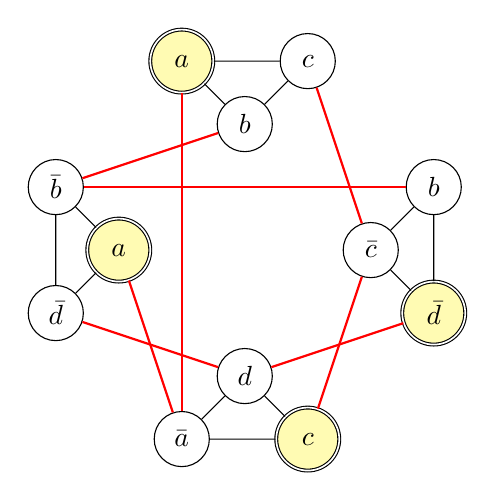
\begin{tikzpicture}[scale=0.8]
          % Define styles for nodes
          \tikzset{
            regular node/.style={circle, draw, minimum size=0.7cm, inner sep=0pt},
            highlighted node/.style={circle, draw, fill=yellow!30, minimum size=0.8cm, inner sep=0pt, double},
          }
          
          % Position nodes in an octagonal arrangement
          % Top nodes
          \node[highlighted node] (a) at (0,4) {$a$};
          \node[regular node] (c1) at (2,4) {$c$};
          \node[regular node] (b1) at (1,3) {$b$};
          
          % Left side nodes
          \node[regular node] (bbar) at (-2,2) {$\bar{b}$};
          \node[highlighted node] (a2) at (-1,1) {$a$};
          \node[regular node] (dbar) at (-2,0) {$\bar{d}$};
          
          % Right side nodes
          \node[regular node] (b2) at (4,2) {$b$};
          \node[regular node] (cbar) at (3,1) {$\bar{c}$};
          \node[highlighted node] (dbar2) at (4,0) {$\bar{d}$};
          
          % Bottom nodes
          \node[regular node] (abar) at (0,-2) {$\bar{a}$};
          \node[highlighted node] (c2) at (2,-2) {$c$};
          \node[regular node] (d) at (1,-1) {$d$};
          
          % Draw black edges (regular connections)
          \draw (a) -- (b1);
          \draw (b1) -- (c1);
          \draw (a) -- (c1);

          \draw (bbar) -- (a2);
          \draw (a2) -- (dbar);
          \draw (bbar) -- (dbar);

          \draw (b2) -- (cbar);
          \draw (cbar) -- (dbar2);
          \draw (b2) -- (dbar2);

          \draw (abar) -- (c2);
          \draw (abar) -- (d);
          \draw (d) -- (c2);
          
          % Draw red edges (special connections)
          \draw[red, thick] (bbar) -- (b2);
          \draw[red, thick] (b1) -- (bbar);
          \draw[red, thick] (a) -- (abar);
          \draw[red, thick] (dbar) -- (d);
          \draw[red, thick] (dbar2) -- (d);
          \draw[red, thick] (c1) -- (cbar);
          \draw[red, thick] (c2) -- (cbar);
          \draw[red, thick] (a2) -- (abar);
        \end{tikzpicture}
        \caption{Reduction graph from 3SAT to MIS. } 
        \label{fig:mis_graph}
      \end{figure}

      The graph contains:
      \begin{enumerate}
        \item Four triangles, one for each clause of $\phi$
        \item Red edges connecting complementary literals (e.g., $b$ with $\bar{b}$)
        \item A maximum independent set highlighted in yellow ($\{a, d\}$) of size 4
      \end{enumerate} 

      This independent set corresponds to the satisfying assignment $(a, b, c, d) = (1, \ast, 1, 0)$. 
      \begin{itemize}
        \item $(a \lor b \lor c)$ is satisfied by $a = 1$
        \item $(b \lor \neg c \lor \neg d)$ is satisfied by $d = 0$. 
        \item $(\neg a \lor c \lor d)$ is satisfied by $c = 1$. 
        \item $(a \lor \neg b \lor \neg d)$ is satisfied by $a = 1$. 
      \end{itemize}

      To demonstrate the proof, we assume that this MIS can be solved in polynomial time, so $MIS \in P$. But since $3SAT \leq_p MIS$, this means that $3SAT \in P$, which is a contradiction since $3SAT \in NP-hard$. 
    \end{example} 

  \subsubsection{Minimum Vertex Cover}

    \begin{definition}[Min Vertex Cover]
      Given an undirected graph $G(V, E)$, a \textbf{vertex cover} is a subset $S \subset V$ where for all $(u, v) \in E$, either $u \in S$ or $v \in S$ (or both). The \textbf{minimum vertex cover} problem asks 
      \begin{enumerate}
        \item Given $G$, find a vertex cover of minimum cardinality. 
        \item Given $G$ and constant $K$, does there exist a vertex cover of size $\leq K$? 
      \end{enumerate}
    \end{definition}

    \begin{theorem}[MVC]
      MVC is NP-hard. 
    \end{theorem}
    \begin{proof}
      \textit{Reduction from MIS}. Recall that an independent set is a subset $S \subset V$ s.t. for all $(u, v) \in E$, $u \in S$ or $v \in S$ (but not both). By definition, we can see that $u \in S \iff u \not\in V \setminus S$, and so IS and VCs are related in the following way: 
      \begin{align}
        S \subset V \text{ is a VC} & \iff \forall (u, v) \in E, u \in S \text{ or } v \in S \text{ or both} \\
                                    & \iff \forall (u, v) \in E, u \not\in S \setminus V \text{ or } v \not\in S \setminus V \text{ or both} \\
                                    & \iff V \setminus S \text{ is an IS}
      \end{align}
      Therefore, if $S$ has size $K$, then $V \setminus S$ will have size $N - K$. We assume that a polytime algorithm exists for MVC, so on input $G(V, E)$, we calculate the MVC, call it $M$, and then we return the corresponding MIS $S = V \setminus M$. 

      \textit{Equivalence}. 
      \begin{enumerate}
        \item ($\Rightarrow$) Assuming we have the solution $|S|$ for MVC, we can return true iff $|V| - |S| \geq K$. 
        \item ($\Leftarrow$) Assuming we have the solution $|S|$ for MIS, we can return true iff $|V| - |S| \leq K$. 
      \end{enumerate}
      But this would imply that there exists such a polytime algorithm, implying that $P = NP$, and therefore MVC must be NP-hard by definition. 
    \end{proof}

    \begin{example}[Reduction from Independent Set to Vertex Cover]
      Just take the complement. 
    \end{example}

  \subsubsection{Maximum Clique}

    \begin{definition}[Max Clique]
      Given an undirected graph $G(V, E)$, a \textbf{clique} is a subset of vertices $S \subset V$ s.t. there is an edge between each pair in $S$, i.e. a \textit{complete subgraph}. The \textbf{maximum clique} problem asks 
      \begin{enumerate}
        \item Given $G$, find the clique of maximum cardinality. 
        \item Given $G$ and constant $K$, does there exist a vertex cover of size $\geq K$? 
      \end{enumerate}
    \end{definition} 

    \begin{theorem}[MC]
      Finding the max clique is NP-hard. 
    \end{theorem}
    \begin{proof}
      \textit{Reduction from MIS}. Observe that 

      Let's define the \textbf{edge-complement} of a graph $G$ as $\bar{G} = (V, \bar{E})$ where $\bar{E}$ is the set of edges not in $G$. Then, note that 
      \begin{align}
        S \subset V \text{ is an IS of } G & \iff \forall u, v \in S, (u, v) \not\in E  \\
                                           & \iff \forall u, v \in S, (u, v) \in \bar{E} \\
                                           & \iff S \text{ is a clique of } \bar{G} 
      \end{align}
      Therefore, we can reduce this from MIS by taking input $G$, getting $\bar{G}$ in $O(N + M)$ time, solving the MIS of $\bar{G}$, and returning the size of the max clique of $\bar{G}$ in our assumed polytime algorithm. Therefore, MC is NP-hard. In fact, we have already proved the equivalence at the same time due to the iff conditions, but we state it explicitly for completeness. 

      \textit{Equivalence}. 
      \begin{enumerate}
        \item ($\Rightarrow$) Assuming we have the MIS solution $S \subset G$, then $S$ is the max clique of $\bar{G}$. 
        \item ($\Leftarrow$) Assuming we have the max clique solution $S \subset G$, then $S$ is the MIS of $\bar{G}$. 
      \end{enumerate}
    \end{proof}

    \begin{example}[Reduction of Independent Set to Clique]
      Just take the edge complement. 
    \end{example}

  \subsubsection{Hamiltonian Paths} 

    \begin{definition}[Hamiltonian Path]
      A \textbf{Hamiltonian path} in a directed graph $G$ is a path that visits every vertex exactly once. 
    \end{definition} 

    \begin{theorem}
      Finding the existence of a Hamiltonian cycle of a graph $G$ is NP-hard. 
    \end{theorem}

    \begin{definition}[Hamiltonian Cycle]
      A \textbf{Hamiltonian cycle} in a directed graph $G$ is a cycle that visits every vertex exactly once. 
    \end{definition}

    \begin{theorem}
      Finding the existence of a Hamiltonian cycle of a graph $G$ is NP-hard. 
    \end{theorem}
    \begin{proof}
      \textit{Reduction from VC}. Given an undirected graph $G(V, E)$ and integer $K$, we want to construct a directed graph $H(V^\prime, E^\prime)$, such that $H$ has a Hamiltonian cycle iff $G$ has a vertex cover of size $K$. We construct $H$ in the following. 
      \begin{enumerate}
        \item For each undirected edge $(u, v) \in E$, the directed graph $H$ contains an \textit{edge gadget} containing 4 vertices 
          \begin{equation}
            (u, v, \mathrm{in}), (u, v, \mathrm{out}), (v, u, \mathrm{in}), (v, u, \mathrm{out})
          \end{equation}
          and 6 directed edges 
          \begin{align*}
            & (u, v, \mathrm{in}) \rightarrow (u, v, \mathrm{out}) & 
            & (u, v, \mathrm{in}) \rightarrow (v, u, \mathrm{in}) & 
            & (v, u, \mathrm{in}) \rightarrow (u, v, \mathrm{in}) \\
            & (v, u, \mathrm{in}) \rightarrow (v, u, \mathrm{out}) & 
            & (u, v, \mathrm{out}) \rightarrow (v, u, \mathrm{out}) & 
            & (v, u, \mathrm{out}) \rightarrow (u, v, \mathrm{out})
          \end{align*}

          \begin{figure}[H]
            \centering 
            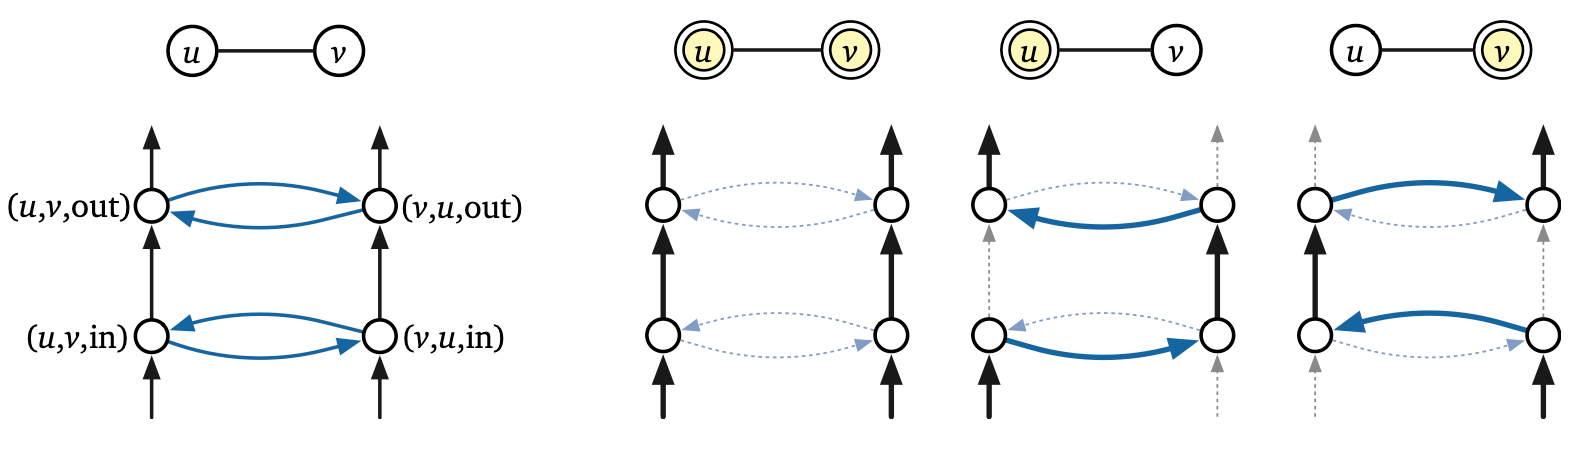
\includegraphics[scale=0.4]{img/edge_gadget.png}
            \caption{An edge gadget and its only possible interactions with a Hamiltonian cycle. Any Hamiltonian cycle in $H$ must pass through an edge gadget in one of 3 ways: straight through on both sides, or with a detour from one side to the other and back. These options will correspond to both $u$ and $v$, only $u$, or only $v$ belonging in the vertex cover.} 
            \label{fig:edge_gadget}
          \end{figure}

        \item For each vertex $u \in V$, all the edge gadgets for incident edges $(u, v)$ are connected in $H$ into a single directed path, called a \textit{vertex chain}. Specifically, suppose vertex $u$ has $d$ neighbors $v_1, \ldots, v_d$. Then $H$ has $d-1$ additional edges $(u, v_i, \mathrm{out}) \rightarrow (u, v_{i+1}, \mathrm{in})$ for each $i = 1, \ldots, d-1$.  

        \item Finally, $H$ also contains $k$ \textit{cover vertices} $x_1, \ldots, x_k$. Each cover vertex has a directed edge to the first vertex in the vertex chain, and a directed edge from the last vertex in each vertex chain. 
      \end{enumerate}

      \textit{Equivalence}. 
      \begin{enumerate}
        \item Suppose that $C = \{u_1, \ldots, u_k\}$ is a vertex cover of $G$ of size $k$. We can construct a Hamiltonian cycle that encodes $C$ as follows. 
        \item Suppose that $H$ contains a Hamiltonian cycle $C$. This cycle must contain an edge from each cover vertex to the start of some vertex chain. 
      \end{enumerate}
    \end{proof}

    \begin{example}[Reduction from Vertex Cover to Directed Hamiltonian Cycle]
      We can see that each double arrowed blue segment represents a pair of directed edges, each part of the gadget. 

      \begin{figure}[H]
        \centering 
        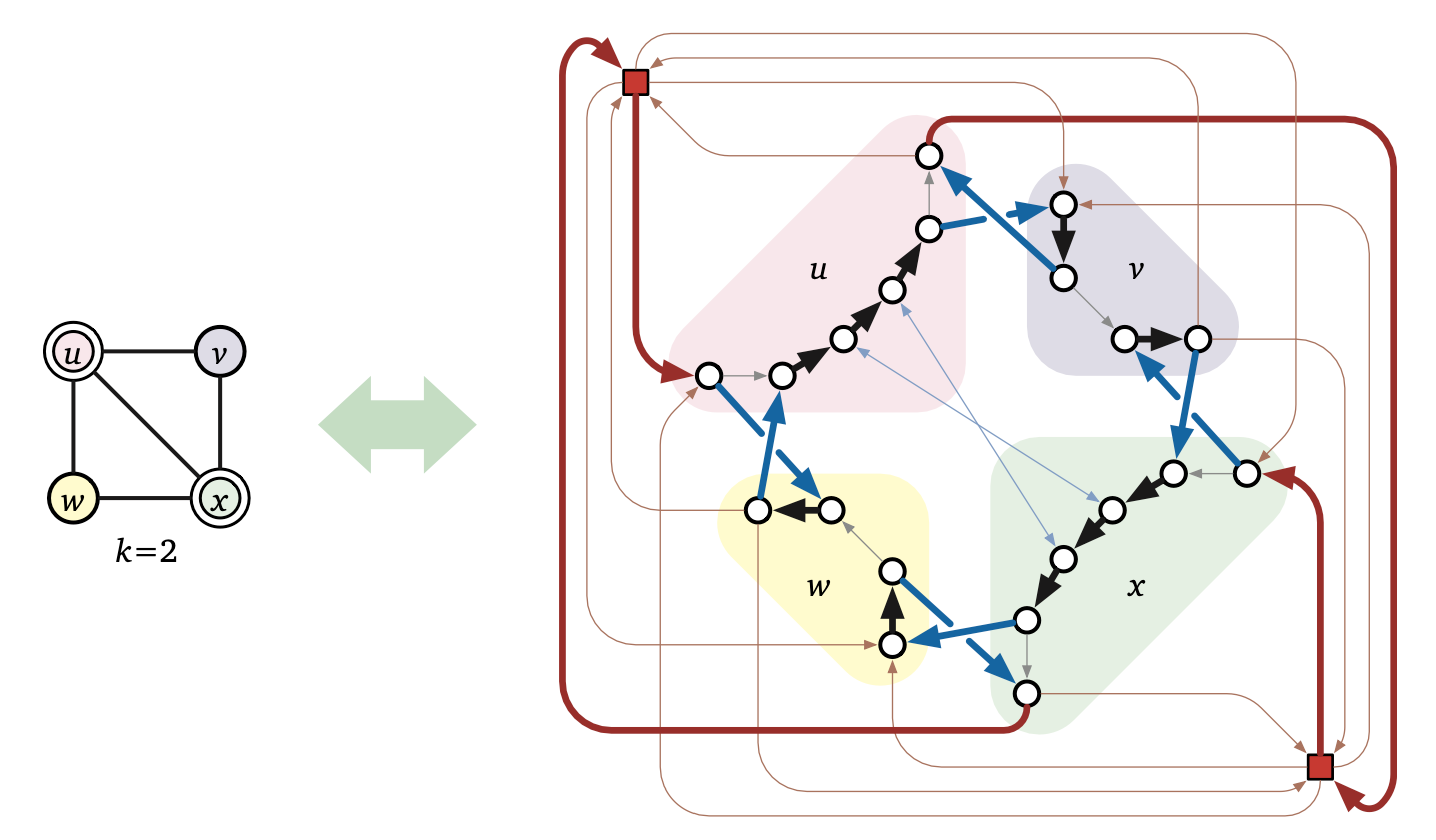
\includegraphics[scale=0.4]{img/ham_reduction.png}
        \caption{Reduction of a simple undirected graph to Hamiltonian cycle.} 
        \label{fig:ham_reduction}
      \end{figure}
    \end{example}

  \subsubsection{Euler Paths}

  \subsubsection{Longest Path}

    \begin{theorem}[Longest Path]
      Finding the longest path in a graph is NP-complete. 
    \end{theorem}

  \subsubsection{Graph Coloring} 

    \begin{definition}[Proper K-coloring]
      A \textbf{proper k-coloring} of a graph $G(V, E)$ is a function $C: V \rightarrow \{1, \ldots k\}$ that assigns one of $k$ colors to each vertex, so that every edge has two different colors at its endpoints. 
    \end{definition}

    \begin{theorem}
      Graph coloring is NP-hard. 
    \end{theorem}
    \begin{proof}
      \textit{Reduction from 3SAT}. 
    \end{proof}

\subsection{Subset Sum}

  \begin{definition}[Subset Sum]
    Given a multiset (allowing duplicates) $X$ of positive integers and a target value $T$, we want to find whether there exists a subset $S \subset X$ that sum up to $T$. 
  \end{definition}

  \begin{theorem}
    Finding the subset sum is NP-hard. 
  \end{theorem}
  \begin{proof}
    \textit{Reduction from MVC}. Given an arbitrary graph $G$ and integer $K$, we need to compute a set $X$ of positive integers and integer $T$, such that $X$ has a subset of sum $T$ iff $G$ has a vertex cover of size $K$. The general idea is that we label each edge with a number in $\{0, 1, 2, 3\}$, where $2$ means that the edge is in the vertex cover. 
    \begin{enumerate}
      \item We label each edge of $G$ from $e = 0, 1, \ldots, E-1$. 
      \item Construct $X = \{\}$: 
      \item for each $e = 0, \ldots, E-1$, add $b_e = 4^e$ to $X$. 
      \item for each vertex $v$, add 
      \begin{equation}
        a_v = 4^{E} + \sum_{e \in \Delta(v)} 4^e
      \end{equation}
      to $X$, where $\Delta(u)$ are the incident edges of $u$. What we have just done is represented each integer in $X$ as an $(E + 1)$ digit number written in base 4. The $E$th digit is $1$ if the integer represents a vertex and $0$ otherwise. For each $e < E$, the $e$th digit is $1$ if the integer represents edge $e$ or one of its endpoints, and $0$ otherwise. 

      \item We set our target sum to be 
      \begin{equation}
        T = K \cdot 4^E = \sum_{e=0}^{E-1} 2 \cdot 4^e
      \end{equation}
      where the first term covers all vertices and the summation covers all edges. 
    \end{enumerate}

    \textit{Equivalence}. 
    \begin{enumerate}
      \item Suppose $G$ has a vertex cover $C$ of size $k$. Consider the subset 
      \begin{equation}
        X^\prime = \{a_v \mid v \in C\} \cup \{b_e \mid \text{edge } e \text{ has exactly 1 endpoint in } C\} 
      \end{equation}
      The sum of the elements in $X^\prime$, written in base 4, has most significant digit $k$ and all other digits equal to $2$. Thus the elements of $X^\prime$ sum exactly to $T$. 

      \item Suppose that there is a subset $X^\prime \subset X$ that sums to $T$. We must have 
      \begin{equation}
        \sum_{v \in V^\prime} a_v + \sum_{e \in E^\prime} b_e = T
      \end{equation}
      for some subset $V^\prime \subset V, E^\prime \subset E$. Then each $b_e$ contributes exactly one digit of $1$ (in base 4). Each edge is incident to 2 vertices, so the non-significant digits contribute two digits of $1$. Therefore, if we sum these base-4 numbers, there are no carries in the first non-sigf $E$ digits since for each $e$ there are only 3 numbers in $X$ whose $e$th digit is $1$. Each edge number $b_e$ contribute only one 1 to the $e$th digit of the sum, but the $e$th digit of $T$ is $2$. Thus, for each edge in $G$, at least one of its endpoints must be in $V^\prime$. In other words, $V^\prime$ is a vertex cover. 
    \end{enumerate}

  \end{proof}

  \begin{example}[Reduction from Vertex Cover to Subset Sum] 
    Given the 4 vertex graph $G$ with $V = \{u, v, w, x\}$ and $E = \{uv, uw, vw, vx, wx\}$, our set $X$ will contain the following base-4 integers. 
    \begin{align*}
      a_u &:= 111000_4 = 1344 & b_{uv} &:= 010000_4 = 256 \\
      a_v &:= 110110_4 = 1300 & b_{uw} &:= 001000_4 = 64 \\
      a_w &:= 101101_4 = 1105 & b_{vw} &:= 000100_4 = 16 \\
      a_x &:= 100011_4 = 1029 & b_{vx} &:= 000010_4 = 4 \\
      & & b_{wx} &:= 000001_4 = 1
    \end{align*} 
    We can see that all the $a$'s have most significant digit $1$, meaning that it represents a vertex, and all the $b$'s that represent an edge are simply stored with a single $1$ and rest $0$s. For the $a$'s, the non-significant digits represent the incident edges. Vertex $u$ has connections to $v, w$, so the next 2 bits, representing the $1$ bits for edges $uv, uw$ are flipped to $1$. If we are looking for a vertex cover of size $K = 2$, we have 
    \begin{equation}
      T = 222222_4 = 2730
    \end{equation} 
    Indeed the vertex cover $\{v, w\}$ corresponds to the subset $\{a_v, a_w, b_{uv}, b_{uw}, b_{vx}, b_{wx}\}$, whose sum is $1300 + 1105 + 256 + 64 + 4 + 1 = 2730$. 
  \end{example}

